\documentclass[12pt, unicode]{beamer}
\usetheme{Warsaw}
\usepackage{luatexja}
\usepackage{color}
\usepackage{listings}
\lstset{
  basicstyle=\ttfamily\bfseries,
  commentstyle=\color{red}\itshape,
  stringstyle=\color{black!30!green},
  showstringspaces=false,
  keywordstyle=\color{blue}\bfseries}
\title{深層学習入門}
\subtitle{深層学習に入門してみた}
\author{Hiroshi Hatake}
\date[2016/07/08]{Technical information sharing seminar}

\begin{document}

\frame{\maketitle}

\begin{frame}{はじめに}
\begin{block}{機械学習とは}
機械学習とは、あるデータセットから特徴量と呼ばれる定量化された指標を抽出し、それらの値を元に未知の入力値から値を取り出すことである。
\end{block}
\end{frame}

\begin{frame}{はじめに}
\begin{block}{噛み砕くと}
あるデータの傾向を繰り返しの計算によって予測し、その予測のパターンに未知の値を当てはめる行為。
\end{block}
\end{frame}

\begin{frame}{はじめに}
\begin{block}{機械学習の流れ}
機械学習の流れ
\end{block}
\onslide<1->
\begin{itemize}
\item<2-> ある既知のデータの集まりを取得する。
\item<3-> 既知のデータの集まりを扱いやすい形に加工する。
\item<4-> 取得したデータの集まりを元に入力値の傾向を反復計算する。
\item<5-> 計算した入力値の傾向を元に、未知の入力値から値を取り出す。
\end{itemize}
\end{frame}

\begin{frame}{背景}
\begin{block}{機械学習の手法}
主にどんな種類のものがあるのか
\end{block}
\onslide<1->
\begin{itemize}
\item 教師あり学習
\item 教師なし学習
\item 教師ありなし混合学習
\item etc.
\end{itemize}
\end{frame}

\begin{frame}{深層学習(Deep Learning)}
\begin{block}{深層学習}
深層学習とは入力の傾向の特徴を学習データから自動で抽出する
\end{block}
\end{frame}

\begin{frame}{深層学習(Deep Learning)}
\begin{block}{深層学習と機械学習の違い}
\onslide<1->
\begin{itemize}
\item<1-> 機械学習では予測に用いる傾向の選び方を人間が決める必要がある
\item<2-> 深層学習では予測に用いる傾向の選び方を自動で獲得する
\end{itemize}
\end{block}
\end{frame}

\begin{frame}{深層学習の解説の前に}
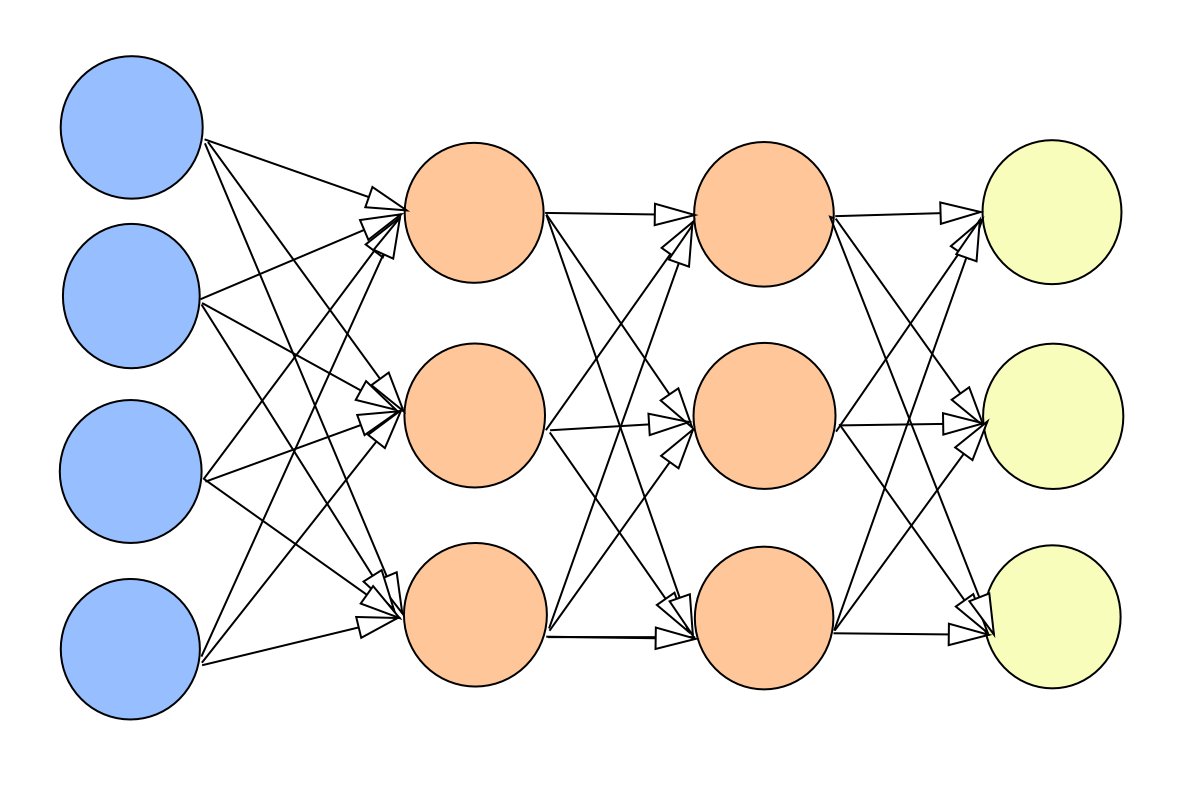
\includegraphics[clip,width=6.5cm]{image/neural_net.png}
\begin{block}{ニューラルネットとは}
\onslide<1->
\begin{itemize}
\item<1-> 値が伝わっていく向きのあるグラフ
\item<2-> グラフの層ごとに重み付けをしたり変換をしたり
\item<3-> グラフ全体を見ると一個の巨大な関数を組み合わせたもの(合成関数とも呼ばれます)
\end{itemize}
\end{block}
\end{frame}

\begin{frame}{深層学習の解説の前に}
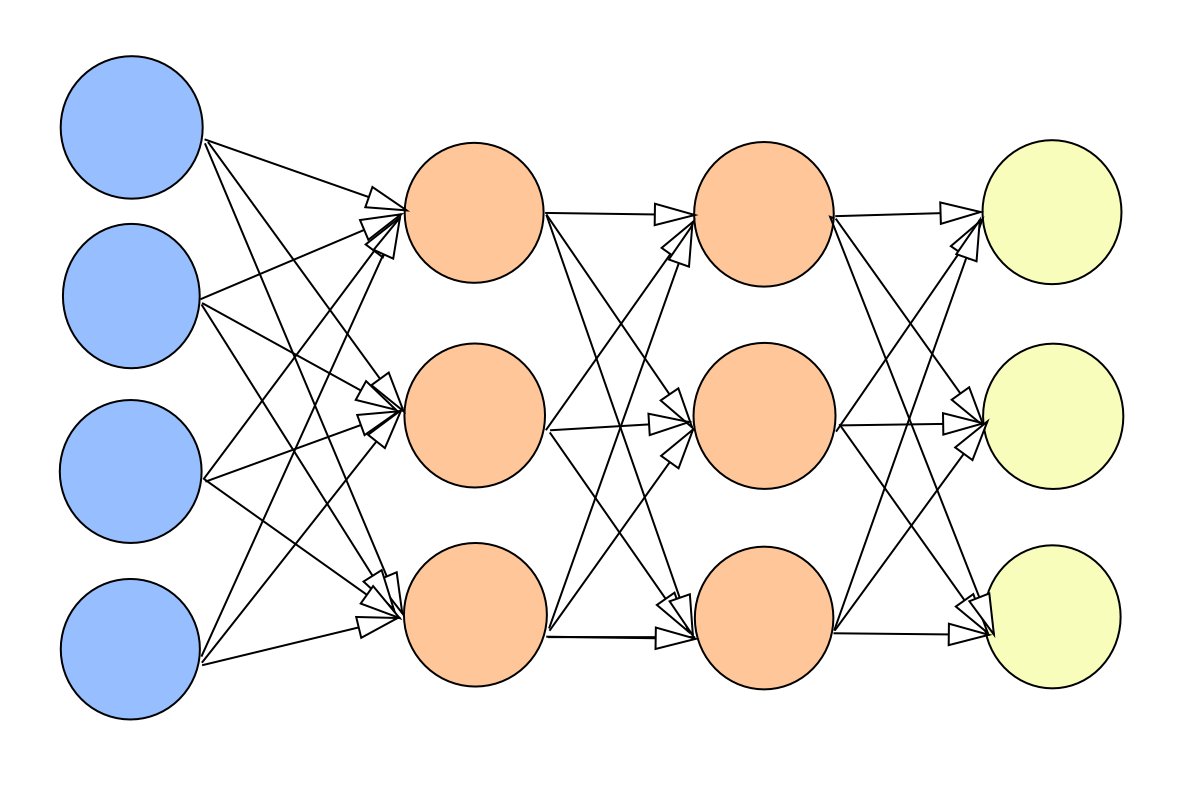
\includegraphics[clip,width=6.5cm]{image/neural_net.png}
\begin{block}{}
このニューラルネットと呼ばれるものを使い、未知の入力値を変換し、目的の値を取り出す。\footnote[frame]{実際にはこのニューラルネットを使う目的関数の設計と勾配の計算、計算したモデルの誤差を定めた誤差関数を最小化する反復計算の手順を踏む。このスライドでは深入りしない。}
\end{block}
\end{frame}

\begin{frame}{深層学習の適用範囲}
\begin{block}{応用範囲}
\onslide<1->
\begin{itemize}
\item<1-> 画像認識
\item<2-> 音声認識
\item<3-> 言語処理
\end{itemize}
\end{block}
\onslide+<4-> どれも非常にデータ量が多くなるタスク
\end{frame}

\begin{frame}{深層学習のフレームワーク}
\begin{block}{フレームワーク}
\begin{itemize}
\item Caffe\footnote[frame]{http://caffe.berkeleyvision.org/}
\item Torch\footnote[frame]{http://torch.ch/}
\item TensorFlow\footnote[frame]{https://www.tensorflow.org/}
\item Chainer\footnote[frame]{http://chainer.org/}
\end{itemize}
\end{block}
\end{frame}

\begin{frame}{Chainer}

\includegraphics[clip,width=1.5cm]{image/chainer_logo.png}
\begin{block}{Chainerとは}
\begin{itemize}
\item CUDAサポートがあり、計算にGPUが使用可能
\item ニューラルネットの設計がPythonのDSLで行え、高い柔軟性がある
\item 値の伝搬のコードだけ書けば、逆誤差伝搬法(backpropagation)\footnote[frame]{勾配を求める手法で、この方法を用いると計算コストを抑えた効率的な計算ができることが知られている。http://neuralnetworksanddeeplearning.com/chap2.htmlなどを参照のこと。}は自動で計算する
\end{itemize}
\end{block}
\end{frame}

\begin{frame}{Chainer}

\includegraphics[clip,width=1.5cm]{image/chainer_logo.png}
\begin{block}{Chainerの特徴}
ニューラルネットの設計。ここは書く必要がある。
\end{block}
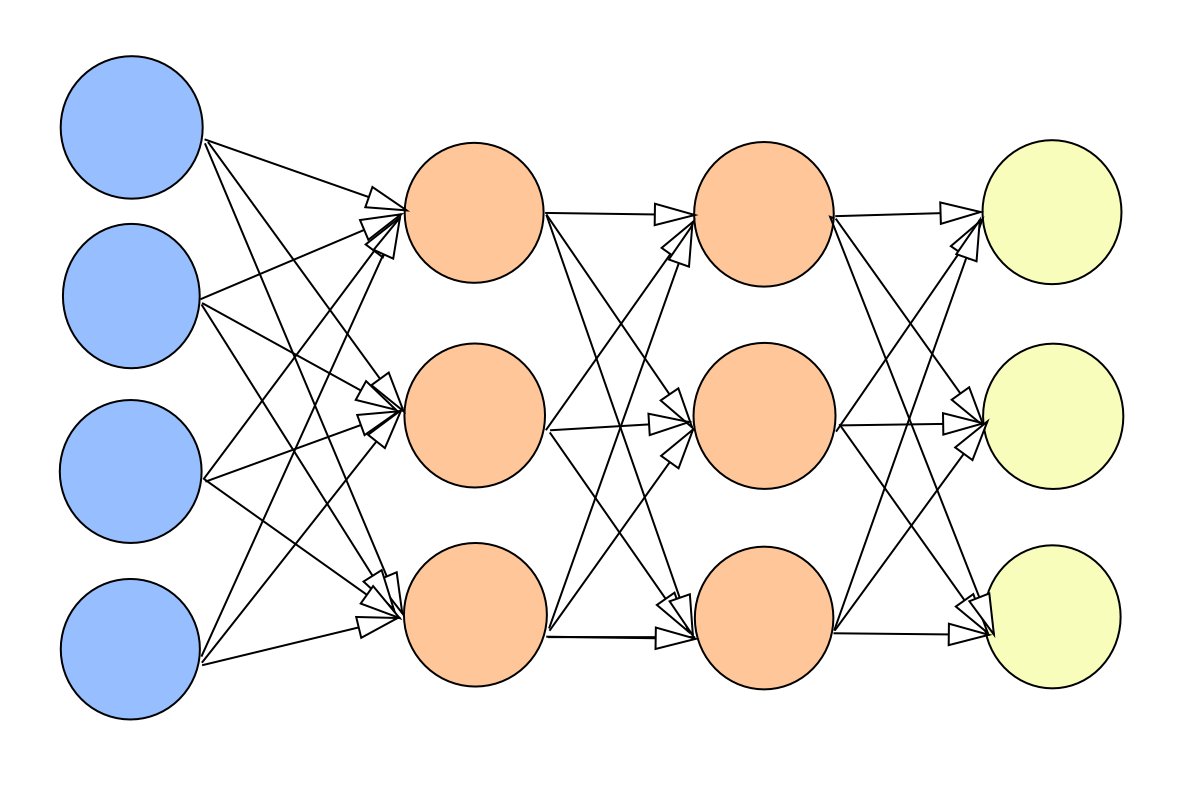
\includegraphics[clip,width=6.5cm]{image/neural_net.png}
\end{frame}

\begin{frame}{Chainer}

\includegraphics[clip,width=1.5cm]{image/chainer_logo.png}
\begin{block}{Chainerの特徴}
backpropagation。ここは自動で計算してくれる。
\end{block}
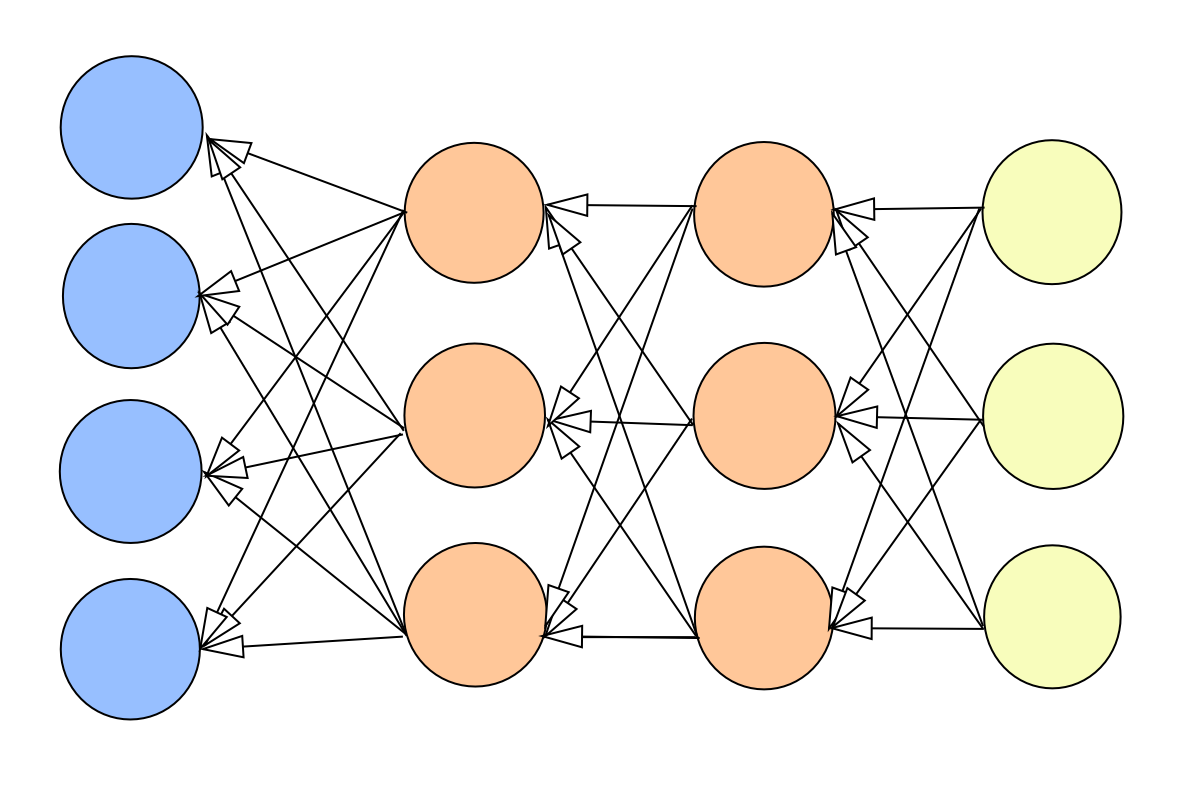
\includegraphics[clip,width=6.5cm]{image/backpropagation.png}
\end{frame}

\begin{frame}{Chainer}

\includegraphics[clip,width=1.5cm]{image/chainer_logo.png}
\begin{block}{Chainerの特徴}
CUDAサポートがある。CUDAとはNVIDIAのGPUの汎用計算環境で、GPUを計算目的に使用することができる。\footnote[frame]{実際はChainerではCuPyとしてNumPyのインターフェースに則ったライブラリからCUDAを使用するようになっている。詳細は http://www.slideshare.net/ryokuta/cupy などを参照のこと。}
\end{block}
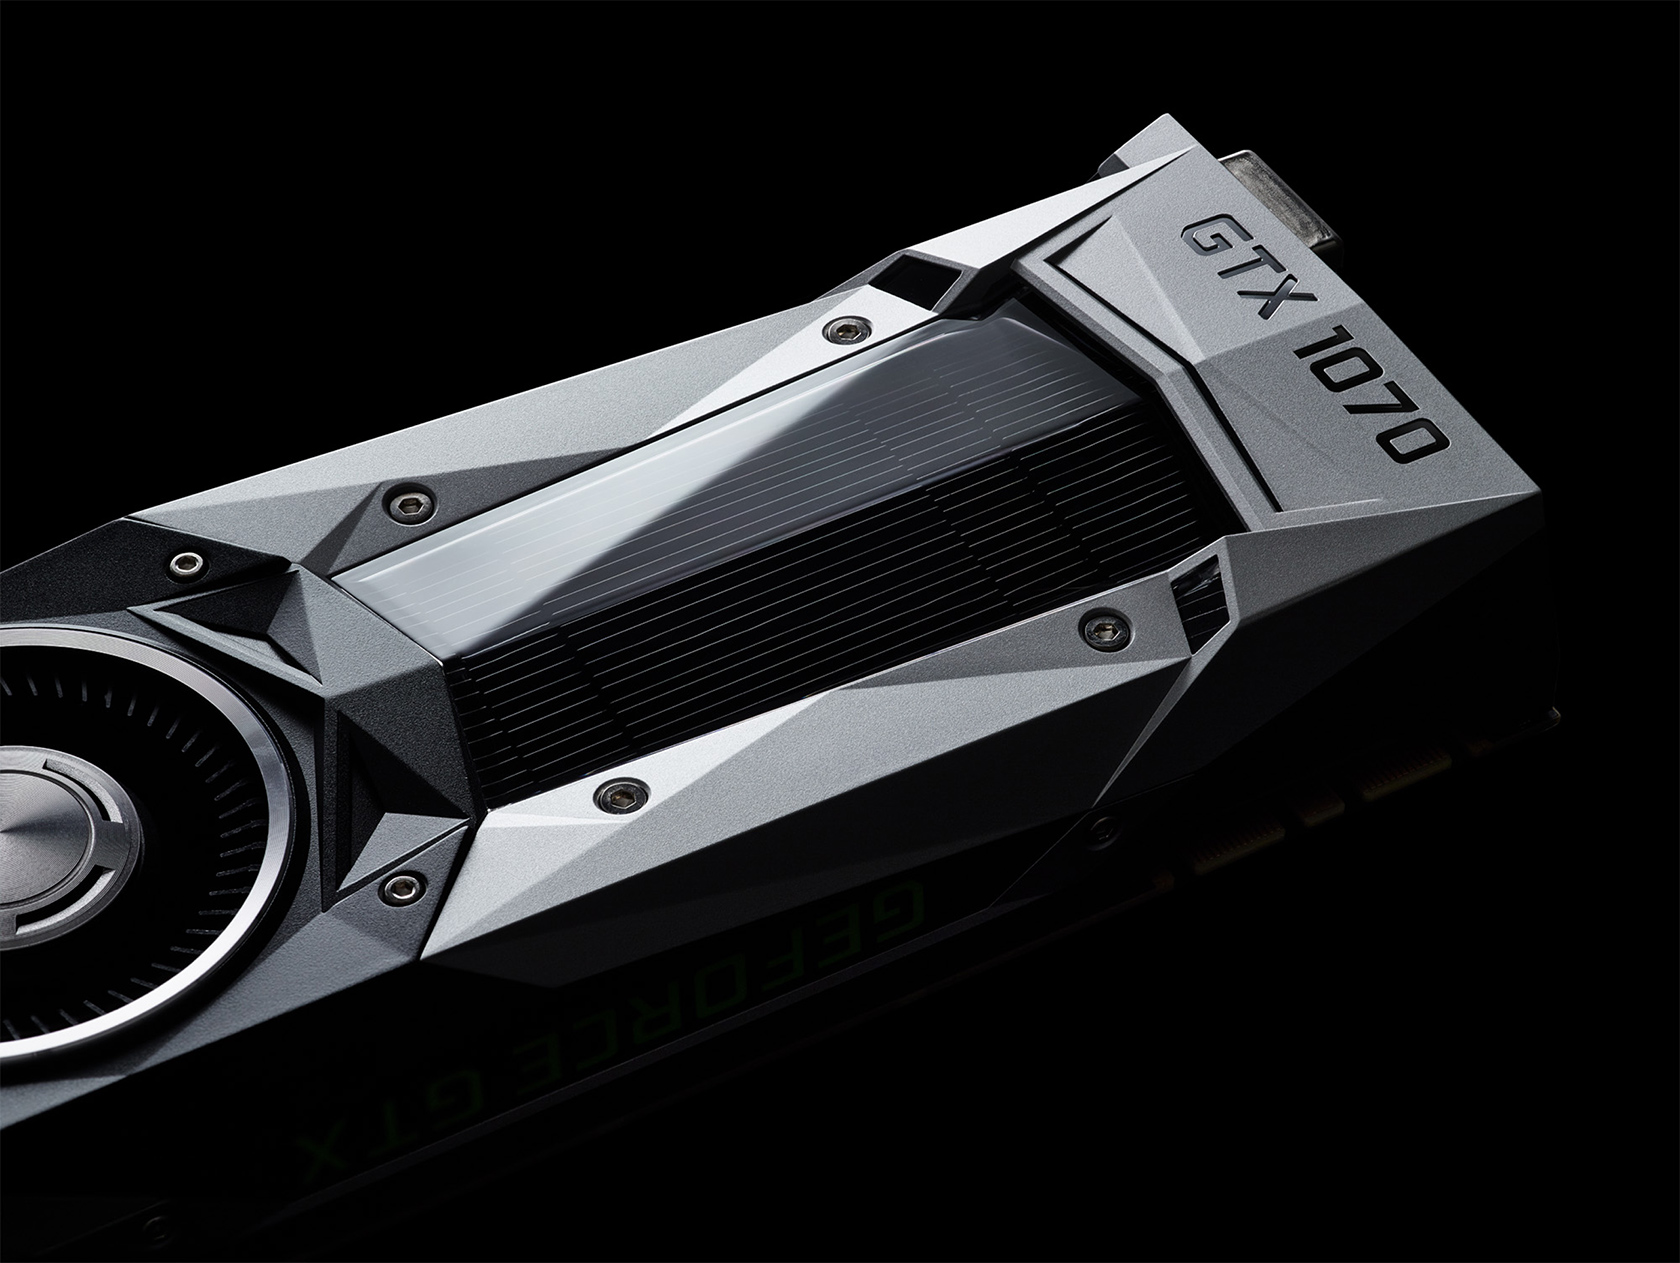
\includegraphics[clip,width=4.0cm]{image/gallery-gtx-1070-4-large.jpg}
\end{frame}

\begin{frame}{Chainerを動かしてみる}

\includegraphics[clip,width=1.5cm]{image/chainer_logo.png}
\begin{block}{Chainerを動作させた環境}
\begin{itemize}
\item OS Ubuntu 14.04.4 LTS
\item Mem 32GB
\item GPU GTX 1070 VRAM 8GB
\item CUDA 8.0RC
\item cuDNN 5.0
\item chainer 1.10
\end{itemize}
\end{block}
\end{frame}

\begin{frame}{応用例1}

\includegraphics[clip,width=1.5cm]{image/chainer_logo.png}
\begin{block}{画風を変換するアルゴリズム}
応用例として画風を変換するアルゴリズムがある。
``A Neural Algorithm of Artistic Stlye''\footnote[frame]{http://arxiv.org/abs/1508.06576}
このスライドではVGGネットワーク\footnote[frame]{http://arxiv.org/pdf/1409.1556}を用いた結果を提示する。
\end{block}
\end{frame}

\begin{frame}{応用例1}

\includegraphics[clip,width=1.5cm]{image/chainer_logo.png}
\begin{block}{画風を変換するアルゴリズム}
スタイル画像とスタイルを適用したい画像を用意する。\footnote[frame]{https://github.com/mattya/chainer-gogh に従って画像のスタイル適用を試しています。}
\end{block}
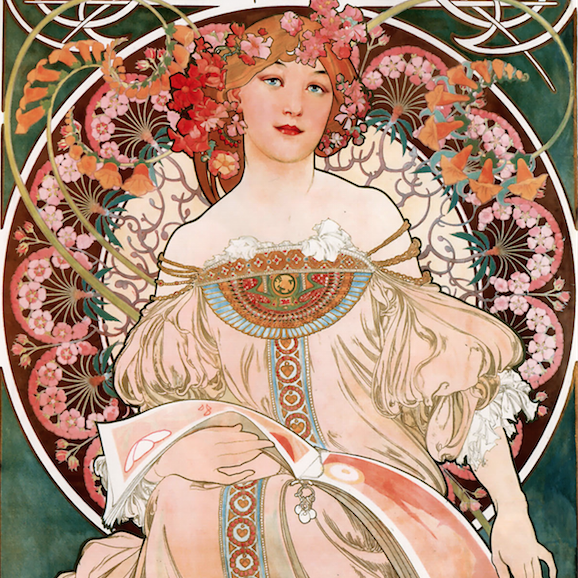
\includegraphics[clip,width=2.0cm]{image/style_6.png}

\includegraphics[clip,width=2.0cm]{image/yuudachi_400x400.png}
・・・→\Large{?}
\end{frame}

\begin{frame}{応用例1}

\includegraphics[clip,width=1.0cm]{image/chainer_logo.png}
\begin{block}{画風を変換するアルゴリズム}
どんどんと誤差関数が小さくなるように計算を回していくと・・・?
\end{block}
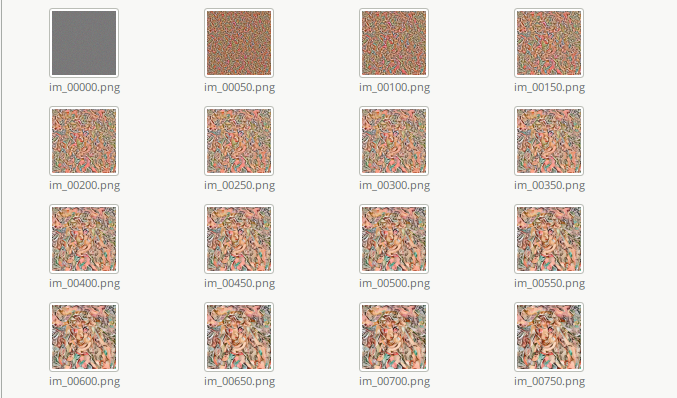
\includegraphics[clip,width=7.0cm]{image/Screenshot1.png}
・・・→\Large{?}
\end{frame}

\begin{frame}{応用例1}

\includegraphics[clip,width=1.0cm]{image/chainer_logo.png}
\begin{block}{画風を変換するアルゴリズム}
どんどんと誤差関数が小さくなるように計算を回していくと・・・?
\end{block}
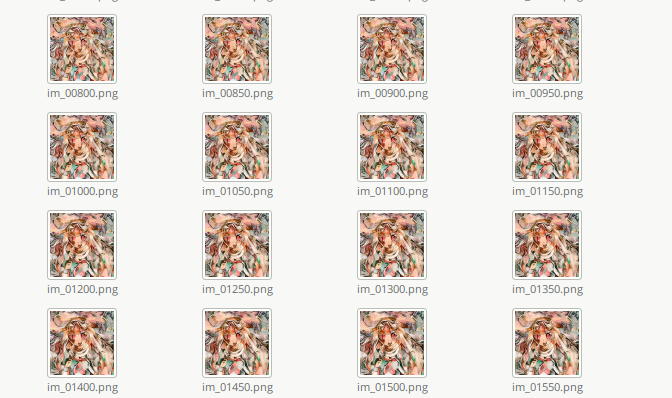
\includegraphics[clip,width=7.0cm]{image/Screenshot2.png}
・・・→\Large{?}
\end{frame}

\begin{frame}{応用例1}

\includegraphics[clip,width=1.0cm]{image/chainer_logo.png}
\begin{block}{画風を変換するアルゴリズム}
どんどんと誤差関数が小さくなるように計算を回していくと・・・?
\end{block}
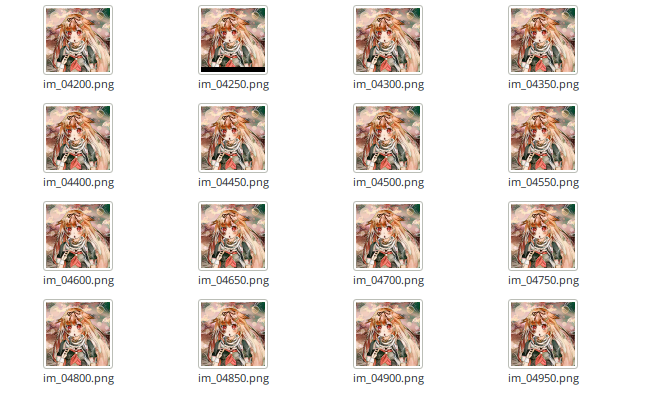
\includegraphics[clip,width=7.0cm]{image/Screenshot3.png}
\end{frame}

\begin{frame}{応用例1−結果}

\includegraphics[clip,width=1.0cm]{image/chainer_logo.png}
\begin{block}{画風を変換するアルゴリズム}
スタイル画像と入力画像、スタイル適用後の画像。
掛かった時間は 313.85秒。パラメータを初期値のまま走らせるとVRAMを2.5GBほど持って行きます。VRAM不足に注意。
\end{block}
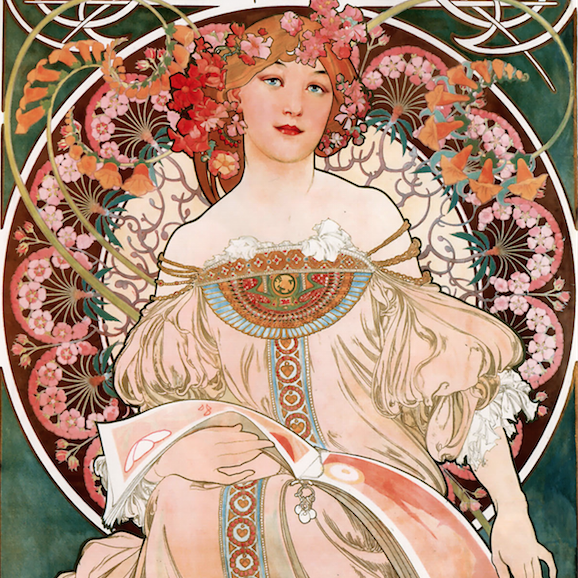
\includegraphics[clip,width=2.0cm]{image/style_6.png}

\includegraphics[clip,width=2.0cm]{image/yuudachi_400x400.png}
・・・→
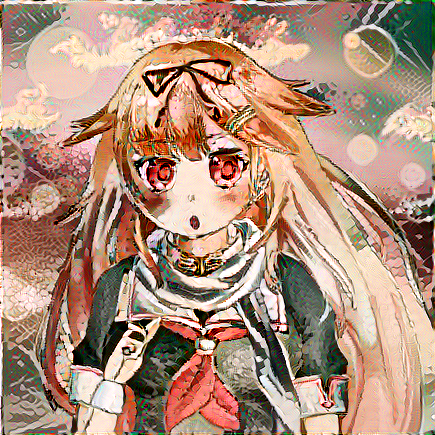
\includegraphics[clip,width=2.0cm]{image/im_04950.png}
\end{frame}

\begin{frame}{応用例1−結果}

\includegraphics[clip,width=1.0cm]{image/chainer_logo.png}
\begin{block}{画風を変換するアルゴリズム}
確かにそれっぽい画像を出力してくれる。…が、GTX 1070でVGGネットワークを用い、CUDAで計算をしても最終的な出力が得られるまで5分強の時間が掛かってしまう。
\end{block}
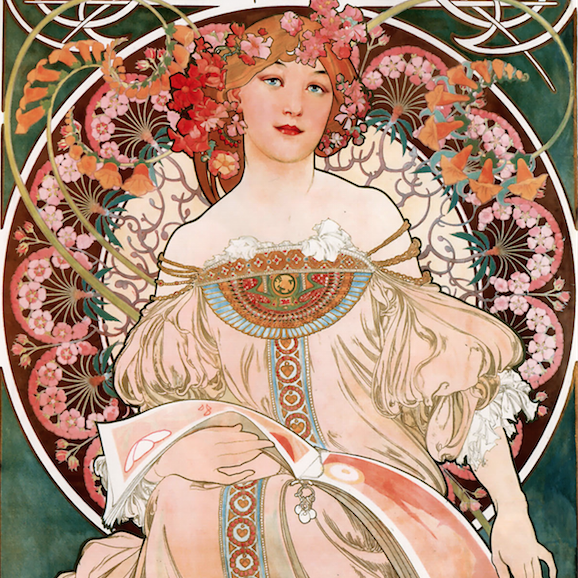
\includegraphics[clip,width=2.0cm]{image/style_6.png}

\includegraphics[clip,width=2.0cm]{image/yuudachi_400x400.png}
・・・→
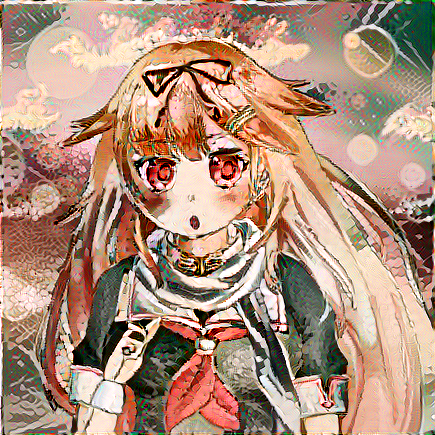
\includegraphics[clip,width=2.0cm]{image/im_04950.png}
\end{frame}

\begin{frame}{応用例1}
\Large{スタイル適用に時間かかりすぎ!}
\end{frame}

\begin{frame}{応用例1}
\Large{スタイル適用だけを速くしたい!}
\end{frame}

\begin{frame}{応用例2}

\includegraphics[clip,width=1.5cm]{image/chainer_logo.png}
\begin{block}{画風を変換するアルゴリズムその2}
応用例として画風を変換するアルゴリズムのその2。
``Perceptual Losses for Real-Time Style Transfer and Super-Resolution''\footnote[frame]{http://arxiv.org/abs/1603.08155}
このスライドではVGGネットワーク\footnote[frame]{http://arxiv.org/pdf/1409.1556}を用いた結果を提示する。\footnote[frame]{https://github.com/yusuketomoto/chainer-fast-neuralstyle に従って画像のスタイル適用を試しています。}
\end{block}
\end{frame}

% Set font size for lstlisting.
\newcommand\Small{\fontsize{9}{9.2}\selectfont}
\begin{frame}[fragile]{応用例2}

\includegraphics[clip,width=1.5cm]{image/chainer_logo.png}
\begin{block}{画風を変換するアルゴリズムその2}
まずはVGGネットに学習をさせてスタイルを適用するニューラルネットを作成する。
また、学習にはMicrosoft COCO dataset\footnote[frame]{http://mscoco.org/dataset/\#download}を用いた。
\end{block}
\begin{lstlisting}[language=bash,basicstyle=\ttfamily\Small,caption={train with style image and dataset}]
$ python train.py -s image/style_6.png -d train2014 \
  -g 0 -o style6
\end{lstlisting}
\end{frame}

\begin{frame}[fragile]{応用例2}

\includegraphics[clip,width=1.5cm]{image/chainer_logo.png}
\begin{block}{画風を変換するアルゴリズムその2}
まずはVGGネットに学習をさせてスタイルを適用するニューラルネットを作成する。
\end{block}
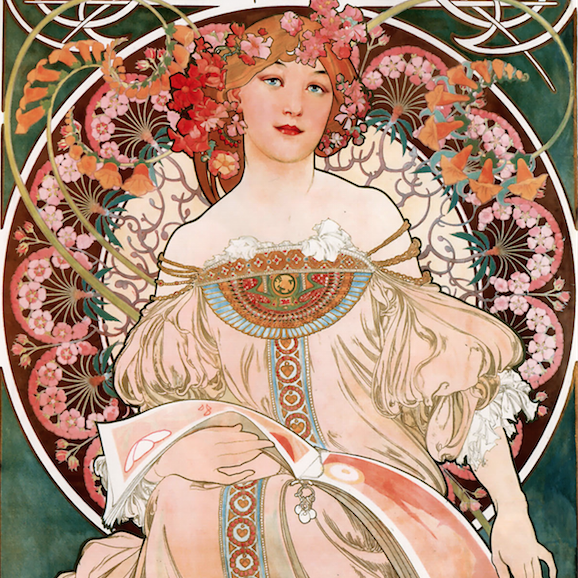
\includegraphics[clip,width=2.0cm]{image/style_6.png}

\includegraphics[clip,width=2.0cm]{image/yuudachi_400x400.png}
・・・→\Large{?}
\end{frame}

\begin{frame}[fragile]{応用例2}

\includegraphics[clip,width=1.5cm]{image/chainer_logo.png}
\begin{block}{画風を変換するアルゴリズムその2}
Microsoft COCO datasetは約8万枚の13GBにもなる画像セット。これを元にスタイルを適用するニューラルネットを作成する。
環境は、先ほどと同一。GTX 1070で2回学習ループを回すのにおよそ4・5時間ほどかかる。\footnote[frame]{はずなのだが、正確な時間を取り忘れた。なぜなら学習にかけてそのまま寝て起きたら終わっていたから。}
\end{block}
\end{frame}

\begin{frame}[fragile]{応用例2}

\includegraphics[clip,width=1.5cm]{image/chainer_logo.png}
\begin{block}{実際に画風を変換するニューラルネットを適用してみる}
学習済みニューラルネットを適用するのはほぼ一瞬。
\end{block}
\begin{lstlisting}[language=bash,basicstyle=\ttfamily\Small,caption={apply trained neural net}]
$ python generate.py sample_image/yuudachi_400x400.png \
  -m models/style6.model \
  -o sample_image/yuudachi_style6.png -g 0
0.949225902557 sec
\end{lstlisting}
\end{frame}

\begin{frame}[fragile]{応用例2}
\Large{0.949225902557 sec}
\end{frame}

\begin{frame}{応用例2−結果}

\includegraphics[clip,width=1.0cm]{image/chainer_logo.png}
\begin{block}{画風を変換するアルゴリズムその2}
確かにそれっぽい画像を出力してくれる。今回は学習済みのモデルを使えば出力が格段に速い。
応用例1比で313.85/0.49≒640.5倍の速さ。およそ3桁倍高速化をしている。(論文中でも ``up to three orders of magnitude faster'' との記述が!)
\end{block}
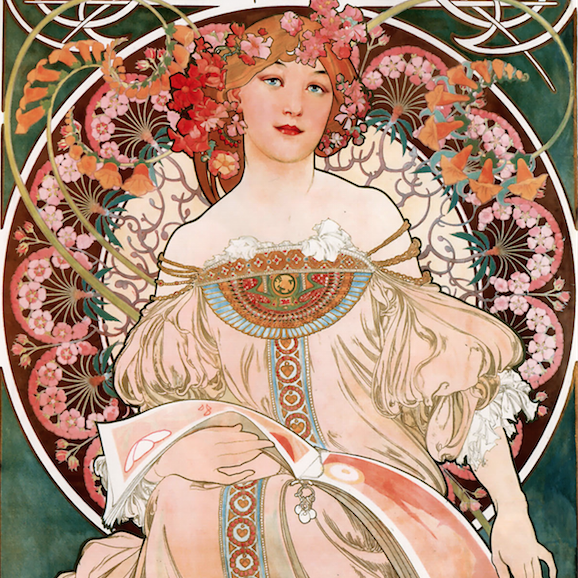
\includegraphics[clip,width=2.0cm]{image/style_6.png}

\includegraphics[clip,width=2.0cm]{image/yuudachi_400x400.png}
・・・→
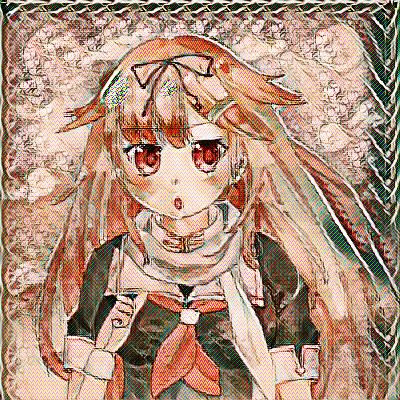
\includegraphics[clip,width=2.0cm]{image/yuudachi_style6.jpg}
\end{frame}

\begin{frame}{まとめ}
\begin{block}{}
\begin{itemize}
\item 学習するときはかなりの計算コストがかかる。
\item このスライドでは省略していますが、計算の裏付けの数式があります。\footnote[frame]{http://bookclub.kodansha.co.jp/product?isbn=9784061529021 がよくまとまっていて詳しい}
\item 定番のニューラルネットをダウンロードしてきてChainerで使える。
\item 実はCaffeなどで作成したモデルもChainerで読み込める!
\item 学習済みの結果を使うときは(使い方にもよりますが)、普通のアルゴリズムと同じように使えます。
\item Chainerはいいぞ。
\end{itemize}
\end{block}
\end{frame}
\end{document}
